% Define the scope, extend, and how of the study
\chapter{Methodology}
\label{chap:methodology}

\begin{note}

WHAT NEEDS TO BE DONE TO ANSWER THE MAIN AND SUB RESEARCH QUESTION

A Prototype VPL is developed to host the functionalities of \ac{GIS} libraries from within an application, and in a composable manner. Additionally, it is used to connect these libraries to various \ac{GUI} features. 
The format of web application is used to allow this prototype to be directly accessible to end users without installation or configuration. 
% Geodata used within the application is also exclusively statically hosted geodata, or user-submitted data. 
This prototype is statically hosted, to minimize operational costs, and is equipped with WebAssembly, so that libraries written in native languages can be used without resorting to active backend web services. 
Finally, as this prototype is intended for \ac{GIS} usage, both scalability to handle sizable datasets, and rich \ac{GUI} support (3D viewers, file inputs, sliders, text boxes, graphs), are primary design considerations and assessment criteria.

So, we are in need of a platform in which:
- Native geocomputation libraries can be directly used by end-users.
- These libraries can be composed into programs

Does a web-based, GUI-rich VPL lead to more \textbf{accessible} and \textbf{composable} native GIS libraries, compared to alternatives?}

How can native GIS libraries be compiled, loaded, and utilized within a static, web-based VPL?

What GUI features are required to facilitate this VPL and these libraries, and to what extend does the web platform aid or hurt these features?

What measures are taken to make this VPL scalable to large geo-datasets, and how effective are these measures?
%  (2. Are the functional properties of a dataflow-VPL uphold by this solution?)

tT what extend does this method "take the best of both software applications and libraries", as described by (SOURCE)?

How does this method compare to existing, alternative VPLs and browser-based geocomputation methods?

\end{note}

This chapter explains the methodology used in this study. 
The overall methodology is to first develop a base VPL (\refsec{sec:method:base-vpl}), followed up by developing a binding system for this VPL (\refsec{sec:method:plugin-system}). 
The final step is to set up and execute a series of tests (\refsec{sec:method:tests}), to analyze the extent to which these implementations solve the various challenges raised by \refchap{chap:intro}.


\section{Characteristics}

This method is characterized by the following properties

\begin{enumerate}[-]
  \item Browser-based usage of native libraries
  \subitem Compilation
  \subitem Loading
  \item Scalability
  \subitem Portability
  \subitem Minimum Abstraction
  \subitem Locality
  \item Rich GUI
  \subitem Geodata visualization
  \subitem parametrization 
\end{enumerate}


\section{Base VPL} 
\label{sec:method:base-vpl}

% The first step of the methodology involves the question: \mySubRQOne.
This implementation is required as a host for all subsequent steps of the methodology. 
While the initial plan was to re-use an existing web VPL, the related works review of \refchap{chap:related} showcased that no exiting browser-based geocomputation VPL would be an appropriate fit.
The Mobius Modeller \citep{janssen_mobius_2021} came closest, but the sizable nature of this project makes aligning its goals with the goals of this study challenging. 
Building a custom implementation would also allow more degrees of freedom, in terms of designing a VPL which takes hosting geocomputation libraries from multiple hosts  into account from the start. 

The following approach was deemed as the most fitting method for implementing this VPL. 
First, the requirements of a dataflow-VPL handling geometry have to be made clear.
Secondly, in order to know what tools may be used to implement this VPl, a small analysis of "widely supported browser features" is made. 
Then, with both these constraints known, a design for a web VPL can be layed out, which can be subsequently implemented. 

\subsection{Requirements}

The requirements of a dataflow-VPL implementation can be subdivided in requirements of a dataflow VPl in general, and a VPL for geo-computation specifically.
Based on the literature study of \refsec{sec:background-vpl}, any dataflow-VPL must at least contain the following aspects: 
\begin{enumerate}[-]
  \item a base 'programming language model'
  \subitem A representation of the 'variables' and 'functions' of the language
  \subitem With all computations being pure functions
  \subitem With all variables being immutable
  \item a 'graph-like' visualization of this data model
  \item an interface to create and edit this graph 
  \item a way to provide input data 
  \item a way to execute the language
  \item a way to display or save output data
\end{enumerate}
The implementation of these aspects would result in a 'baseline', general purpose, dataflow VPL. 
To specialize this implementation further, A visual programming language handling geometry should have:
\begin{enumerate}[-]
  \item Type safety 
  \item A way to load or to create geometry data 
  \item A way to export geometry data
  \item A method to preview geometry data in 3D
  \item A standard set of geometric types and operations
\end{enumerate}
These requirements need further explanation.
First, regarding type safety.
In this context, type safety refers to: 
The input and output of a function should have a type stated, and users should be notified of incorrect usage of types, or 'invalid connections'.
Geometry VPLs in particular need this, as many data representations of geometry are required to be precise about their data usage.
A VPL used to construct geometry should reflect this.
Additionally, when these types are clear and clearly communicated, users must have ways to provide these types as inputs or outputs. 
This will require specialized parsers to become part of the VPL, such as an obj and geojson reader and writers. 

Regarding visualization, A hallmark of dataflow VPLs is the ability to inspect the geometry created in-between steps, so this must be provided for.
This is also a good fit, since the immutable nature of dataflow VPL variables make these variables ideal for caching. 

Finally, a geometry VPL should contain a set of 'internal', basic types and operations.
All aforementioned features are difficult to implement without defining some set of internally recognized data types. 
Basic operations are needed in particular to transform between the types.

% \begin{note}
%   Figure out what to do with this: 
%     Interactivity is the defining factor of the vpl. 
%     a list of standard VPL features & application features required as a base-line:  
%   - Users must be able to construct a script by visual means.

\subsection{Widely supported browser features}

\begin{figure}
  \centering
  \graphicspath{ {../../assets/plots/browser-usage/} }
  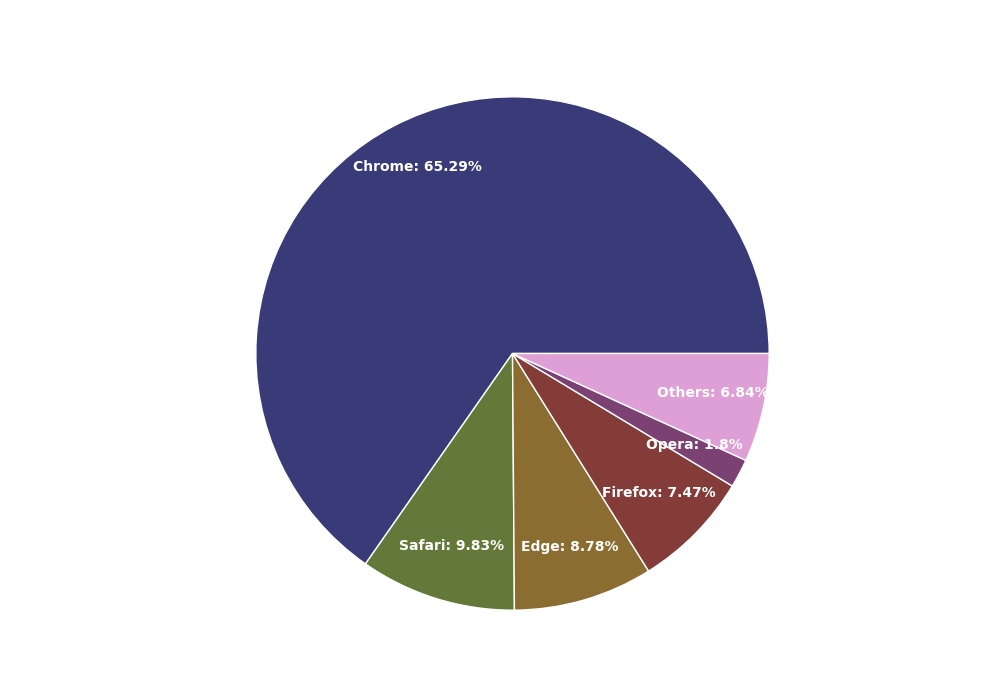
\includegraphics[width=0.7\linewidth]{plot.png}
  \caption[Browser usage]{Fall 2021 desktop browser usage statistics. Data averaged over (\citep{dashiki_simple_2020,w3counter_global_2020,the_netmarketshare_team_browser_2020,statcounter_global_stats_browser_2020})}
  \label{fig:browser-usage}
\end{figure}

This study defines "widely supported browser features" as the set of default features implemented by the browser engines of 'major browsers'. 
Based on the desktop browser market shares of \reffig{fig:browser-usage}, the chromium based browsers (Chrome, Edge, Opera) have the majority. 
This is followed up by Firefox, based on the Gecko engine, and Safari, based on webkit. 
By supporting these three engines, the vast majority of end-users can be served.

The set of features common in these three browser engines are well-documented on websites like MDN web docs \citep{mozilla_mdn_2022}. 
This set includes the following features relevant for the 3D VPL:
\begin{enumerate}[-]
  \item WebGL \& WebGL2 (WebGPU is not fully covered yet)
  \item 2D Canvas API
  \item Web Workers
  \item Web Components
  \item WebAssembly
\end{enumerate}

\subsection{Design}

% \begin{note}
%   TODO: MAKE SOME UML DIAGRAMS
% \end{note}

A software application of a VPL adhering to the specifications mentioned can be implemented in several ways. 
The design chosen is a \ac{MVC} setup written in javascript.  
The \ac{MVC} is a common model for interface-focussed applications, and allows us to reason about the model of the VPL language an a separate level from the editor / viewer.
The JavaScript language will be used instead of webassembly alternatives, in order to limit the usage of webassembly to just the libraries. 
Using WebAssembly too much at too many different locations will make the results of this study less clear.

Javascript is a multi-paradigm language.
This study chose an object-oriented approach, and will use some of the design patterns layed out in \citep{gamma_design_1994}.
This design is further elaborated in the subsequent sections, first by covering the Shim classes, followed up by design details corresponding to the model, view and controller:

\subsubsection*{Shim Types}

\begin{figure}
  \centering
  \graphicspath{ {../../assets/images/implementation/} }
  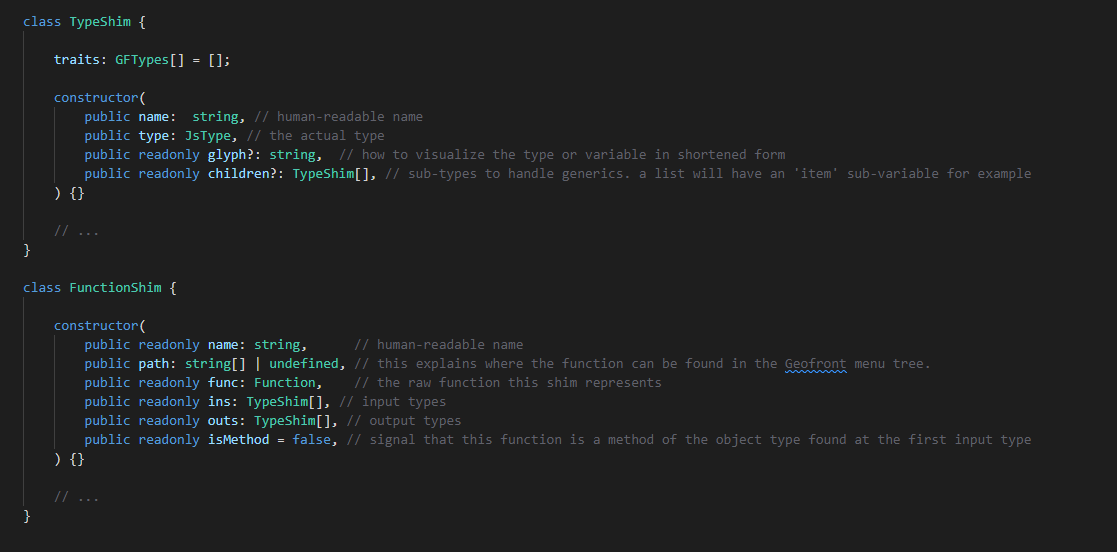
\includegraphics[width=\linewidth]{shim-uml.png}
  \caption[Shim Classes]{Shim classes. (pseudo) code is presented instead of a UML diagram, to be clear about the recursive aspects. (TODO: add modules) }
  \label{fig:shim-classes}
\end{figure}

Firstly, since a VPL is partially a programming language, a model is needed to reason about some of the features of a programming language, such as functions, types, variables, and modules / libraries / plugins.
For example, we desire to store a description of a function, how many input parameters it needs, and which variable types each input requires. 

These needs led to the design of classes serving as equivalents of these language features, called shims. 
\reffig{fig:shim-classes} shows a type-shim and function-shim respectively. 
A Shim equivalents of a module, and a VPL graph are also required. 

The shim classes are designed using the Object Type design pattern \citep{gamma_design_1994}. 
This means that these objects are used as types. 
For example, a loaded function corresponds to exactly one \m{FunctionShim} instance, and that this instance is shared as a read only with any object wishing to eventually use the function. 
% the \m{FunctionShim} offers the name, description, number of inputs, and number of outputs of a function, as well as ways to invoke the function it represents.
This is also useful for defining recursive types. 
TypeShims can be structured recursively to define a \m{List of List of strings} for example. 



\subsubsection*{Model}
\label{sec:method-model}

\begin{figure}
  \centering
  \graphicspath{ {../../assets/images/misc/} }
  
\includegraphics[width=\linewidth]{placeholder.png}
  \caption[Shim Classes]{(TODO: MAKE A DAG UML)}
  \label{fig:dag-model}
\end{figure}

From the Shims, the main model of a VPL script can be conceived (see \reffig{fig:dag-model}). 
This model is at its core a \ac{DAG}. 
This \ac{DAG} should be a object-oriented, graph-like representation of the data flow of a regular programming language. 
This design can be implemented by writing a \m{Graph} class, containing \m{Node} and \m{Cable} objects. 

In this model, Nodes are analogous to function \emph{invocations} of normal programming languages. 
As such, a Node knows about the function they represent through a \m{FunctionShim} reference. 
The node contains a number of input and output sockets based on this information, and each socket contains exactly one optional reference to a \m{Cable}.  
As the name implies, these Nodes form the nodes of the DAG. 
However, they differ from a pure DAG implementation, in that they also provide pointers back in the reverse direction, forming essentially a normal graph, or a doubly linked list. 
This is required for keeping track of all references pointing to a Node, so that upon the deletion of a node, all pointers can quickly be identified and nullified.

The Cables of this model are an analogy to the variables of regular languages. 
Cables know about the type they represent through a \m{TypeShim}. 
A Cable must have exactly one origin, which is an output socket of a Nodes, 
and must have one or more destinations, which are the input sockets of other Nodes.
This is required for the same reasons as the doubly linked nature of the Cables. 
 
To reason about the graph as a whole, a overarching \m{Graph} class will be needed.
This is what would be called a 'program' or 'script' in a regular language. 
Because of the way Cables and Nodes reference each other, the graph has characteristics of a doubly linked list data structure. 
Using normal references in these types of situations could easily lead to memory management issues such as Dangling Pointers.
For this reason, centralizing the graph logic is desirable over adding complex logic to individual Nodes. 
This will make it possible to substitute references with id integers to prevent these types of problems. 



\subsubsection*{View}
\label{sec:method-view}

The view aspect of the VPL will require three main components. 
First, the graph itself will need to be visualized in some manner.
A graph based visualization will be used, based on the node-cable connections of the graph model. 
Important to this view is that it will need to be redrawn often. 
Users will want to add, select, change, and delete nodes, and these interactions should be clearly represented. 
This makes the HTML5 'canvas API' an ideal fit to this component.

Secondly, since not all actions and interactions will be done by clicking on the graph itself, a \ac{GUI} surrounding this graph visualization is required.
This will also need to house common application features, like 'new', 'save', 'load', 'export', etc.  
The browser context means that this aspect will need to be facilitated by HTML. 
Styling is required to make what is essentially a website look and behave like an application. 

Finally, the VPL requires some way of visualizing 3D geometry, so that in-between products containing spatial data can be viewed. 
a custom 3D engine, specialized to the needs of the VPL, would be best option for this aspect.

\subsubsection*{Controller}
\label{sec:method-controller}

Finally, a controller will be needed to modify and manipulate the VPL.
It will need to house all types of interactions, such as loading and saving a VPL script, model manipulation and updating the view only when necessary.
Two important aspects require further explanation: Keeping track of history, and calculating the graph. 

\emph{History}

In order to support all these interactions, especially undo / redo support, we are required to explicitly track the history of the graph. 
A Command Pattern \citep{gamma_design_1994} makes for a good fit in this regard.
Instead of directly editing the graph, all manipulation actions should be represented as \m{Action} objects. 
Each Action can 'do' and 'undo' a specific action, and the data needed to make this do and undo are stored within the action. 
By then introducing a \m{Bridge} class, the model and controller can be separated, only allowing interaction with the model by serving this bridge Action objects. The \m{Bridge} maintains a stack of undo and redo actions, which represents this history.  

% Additionally, editing any graph data structure is never trivial. 
% Special care must be taken to ensure the validity of a graph before and after changes, and is especially the case with Geofront's Doubly linked graph. 
% To the best of the authors knowledge, these is no "trick" or "pattern" to ease this. Instead, the Graph and Graph Decoupler classes both have been designed in such a way 

\emph{Calculation}

When regarding the graph model, or any other programming language, we see many functions requiring variables which are the result of other functions. 
This is why a graph like this can also be called a dependency graph. 
If one wishes to calculate the result of a VPL script, then these dependencies must be taken into account. 
The functions the graph muse be sorted in such a way that all dependencies are known before a function is calculated.
Such a problem is known as a topological sorting problem, and can be solved using Kahn's algorithm (\refsec{fig:kahn}): 

\begin{figure}
  \centering
  \begin{lstlisting}
    Step -1: 
      Make an `order` list
    Step 0: 
      Make a `visisted` counter, initialized at 0
    Step 1: 
      Make a `dependency` counter for each node, initialized at 0
    Step 2: 
      Add 1 to this counter for each input edge of this node.
    Step 3: 
      Fill a queue with all dependency 0 nodes. 
      These are the starter nodes.
    Step 4: 
      Remove a node from the queue (Dequeue operation) and then:
      add the nodes' id to the `order` list.
      Increment `visisted` counter by 1.
      Decrease `dependency` counter by 1 for all dependent nodes.
      If one `dependency` counter reaches 0, 
        add it to the queue.
    Step 5: 
      Repeat Step 4 until the queue is empty.
    Step 6: 
      If `visisted` counter is not equal to the number of nodes, 
        then the graph was degenerate, and probably cyclical. 
    \end{lstlisting}
  \caption[Kahns algorithm]{Khan's algorithm in pseudo code}
  \label{fig:kahn}
\end{figure}

Using this algorithm for calculating a VPL has several important qualities. 
First of all, it detects cyclical graph patterns without getting trapped within such a loop. 
VPLs implemented on the basis of an event-system suffer from this drawback, and models such as those must continuously check their own topology to avoid loops. 

Secondly, by sorting the \emph{order} of calculation before actually performing the calculations, we can use the algorithm for more than just the calculation.
For example, in theory this could be used to compile a VPL Script to Javascript at runtime, by composing a list of functions based on this order. 

Finally, if all intermediate calculation results are cached, this same algorithm can also be used for performing partial recalculations of the graph. 
The starting positions of the algorithm then simply become the altered parameter, after which only the invalidated functions will recalculate. 

\emph{Mutability}

Recall that a variable in this VPL model always has one origin, and one or multiple destinations, just like variables a regular language.
The calculation system requires to know the mutability of the destination function parameters. 
This has two reasons.
First, to allow concurrent calculations, all functions using a variable should only be allowed to use a immutable references to this variable, in order to prevent data races. 
And secondly, to prevent unnecessary copies of variables, only one function should be allow to 'claim ownership' of a variable, as in, modify the data and pass it along as output, or delete it and free the memory. 
This is inspired by the Rust language model \citep{contributors_what_2022}. 
In such a system, concurrency can still occur between all other immutable references to this variable.
However, only when all these calculations are done, may this final transformative step occur.

All this to say, the mutability of function parameters must be known in order to create a performant and memory efficient graph calculation system.  

% \begin{note}
%   TODO: this requires follow up, and a graphic illustration
% \end{note}


% \subsection*{C: Implementation Steps}

% \begin{note}
% TODO: An image showing the phases of development
% \end{note}

% To find the answer to question C, this study implemented the core of the prototype \ac{geo-web-vpl}.
% Just like the entire study, the development trajectory for implementing will be done incrementally, ensuring results during all steps of the development. 
% The first step of the phase consists of creating the basics of the \ac{gui} itself. 
% A basic \ac{vpl} will be created which can only process boolean statements. 
% The second step involves developing the main datamodel of the VPL, to represent the program in an object-oriented way. 
% The third step adds types, geometry, and the visualization of this geometry in 3D, as well as textures / images in 2d. \
% The fourth step adds geospatial data support, and adds Web Feature Services, Web Map Services, and coordinate reference systems.  

%%%%%%%%%%%%%%%%%%%%%%%%%%%%%%%%%%%%%%%%%%%%%%%%%%%%%%%%%%%%%%%%%%%%%%%%%%%%%%%%%%%%%%%%%%%%%%%%%%%%%%%%%%%%%%
%%%%%%%%%%%%%%%%%%%%%%%%%%%%%%%%%%%%%%%%%%%%%%%%%%%%%%%%%%%%%%%%%%%%%%%%%%%%%%%%%%%%%%%%%%%%%%%%%%%%%%%%%%%%%%
%%%%%%%%%%%%%%%%%%%%%%%%%%%%%%%%%%%%%%%%%%%%%%%%%%%%%%%%%%%%%%%%%%%%%%%%%%%%%%%%%%%%%%%%%%%%%%%%%%%%%%%%%%%%%%
%%%%%%%%%%%%%%%%%%%%%%%%%%%%%%%%%%%%%%%%%%%%%%%%%%%%%%%%%%%%%%%%%%%%%%%%%%%%%%%%%%%%%%%%%%%%%%%%%%%%%%%%%%%%%%
%%%%%%%%%%%%%%%%%%%%%%%%%%%%%%%%%%%%%%%%%%%%%%%%%%%%%%%%%%%%%%%%%%%%%%%%%%%%%%%%%%%%%%%%%%%%%%%%%%%%%%%%%%%%%%
\newpage
\section{Plugin System} 
\label{sec:method:plugin-system}

The second step of the methodology involves developing a method to use libraries from native sources within the VPL outlined above. 
% This aspect of the methodology seeks to design a base to answer the questions: \mySubRQTwo and \mySubRQThree.

The plugin system refers to the combination of the plugin model these libraries will need to adhere to, together with the importer of those libraries in the VPL. 
This section will cover the design of both, as well as the proposed compilation workflow.

% to what extent can a web-consumable library be loaded into a web-vpl without explicit configuration?

\subsection{Terminology}

Firstly, some confusion exists between 'libraries' and 'plugins'.
The distinction between them is relevant to the design of the plugin system. 
Typically, one would use the terminology 'libraries' and 'bindings' when referring to expanding the functionality of a codebase with a 'package of functions'.
One would use 'plugins' when referring to practically the same phenomena, but within the context of an application.

With a VPL being something in between a programming language and an application, it remains difficult to determine the appropriate terminology.  
This is further complicated if a plugin is able to double as a library, as will be explained.

\subsection{Requirements}

First and foremost, in order to use software libraries written in system-level languages in a web browser, these libraries will need to be compiled to the WebAssembly binary format (see \refsec{sec:background-wasm}). 
Secondly, in order to use these binaries on a VPL canvas, they must include some explanation of how to expose its inner functionality as VPL visual components.
Thirdly, the core design goal for the plugin system is library portability.
Portability in this context refers to: "usable in multiple locations".
As such, the native geocomputation libraries we seek to support must not only be compiled to a format usable in a web-based VPL, but to a format usable on the web as a whole. 
And finally, the full workflow of bringing a geo-library to the web VPL should be as automated as possible. 

\newpage
\subsection{Design}

These requirements lead to the following design for the plugin system.
Both the model of what a plugin should look like, and the plugin loader on the side of the VPL must be designed in conjunction, to make sure the models match.  
The plugin model:
\begin{enumerate}[-]
  \item Must wrap a geocomputation library compiled with WebAssembly.
  \item Must include optional metadata about how the library may be used in the VPL.
  \item Must be packaged as a regular javascript library.
  \item Must be distributed using a \ac{CDN} like the Node Package Manager (NPM).
\end{enumerate}

Furthermore, the plugin loader of the VPL must be able to: 
\begin{enumerate}[-]
  \item accept a regular javascript library as a plugin. 
  \item load exposed metadata about all included logic.
  \item convert this to an internal representation of a library.
\end{enumerate}

This system utilizes the infrastructure of regular javascript libraries as much as possible. 
This way, existing javascript tooling, such as \ac{CDN}s, can be utilized for distribution, updates and version control.
Additionally, this setup addresses the portability requirement by making these libraries interoperable with unaffiliated projects on both the frontend and backend (see \reffig{fig:plugin-model}).
It might even allow libraries to be loaded which were never intended to be used by the VPL.

For the scope of this system, we will refer to a native geo-library wrapped with the appropriate VPL / javascript bindings as a 'plugin', even though these projects are javascript libraries, and can be loaded as a library into regular javascript projects. 

\begin{figure}
  \centering
  \graphicspath{ {../../assets/diagrams/} }
  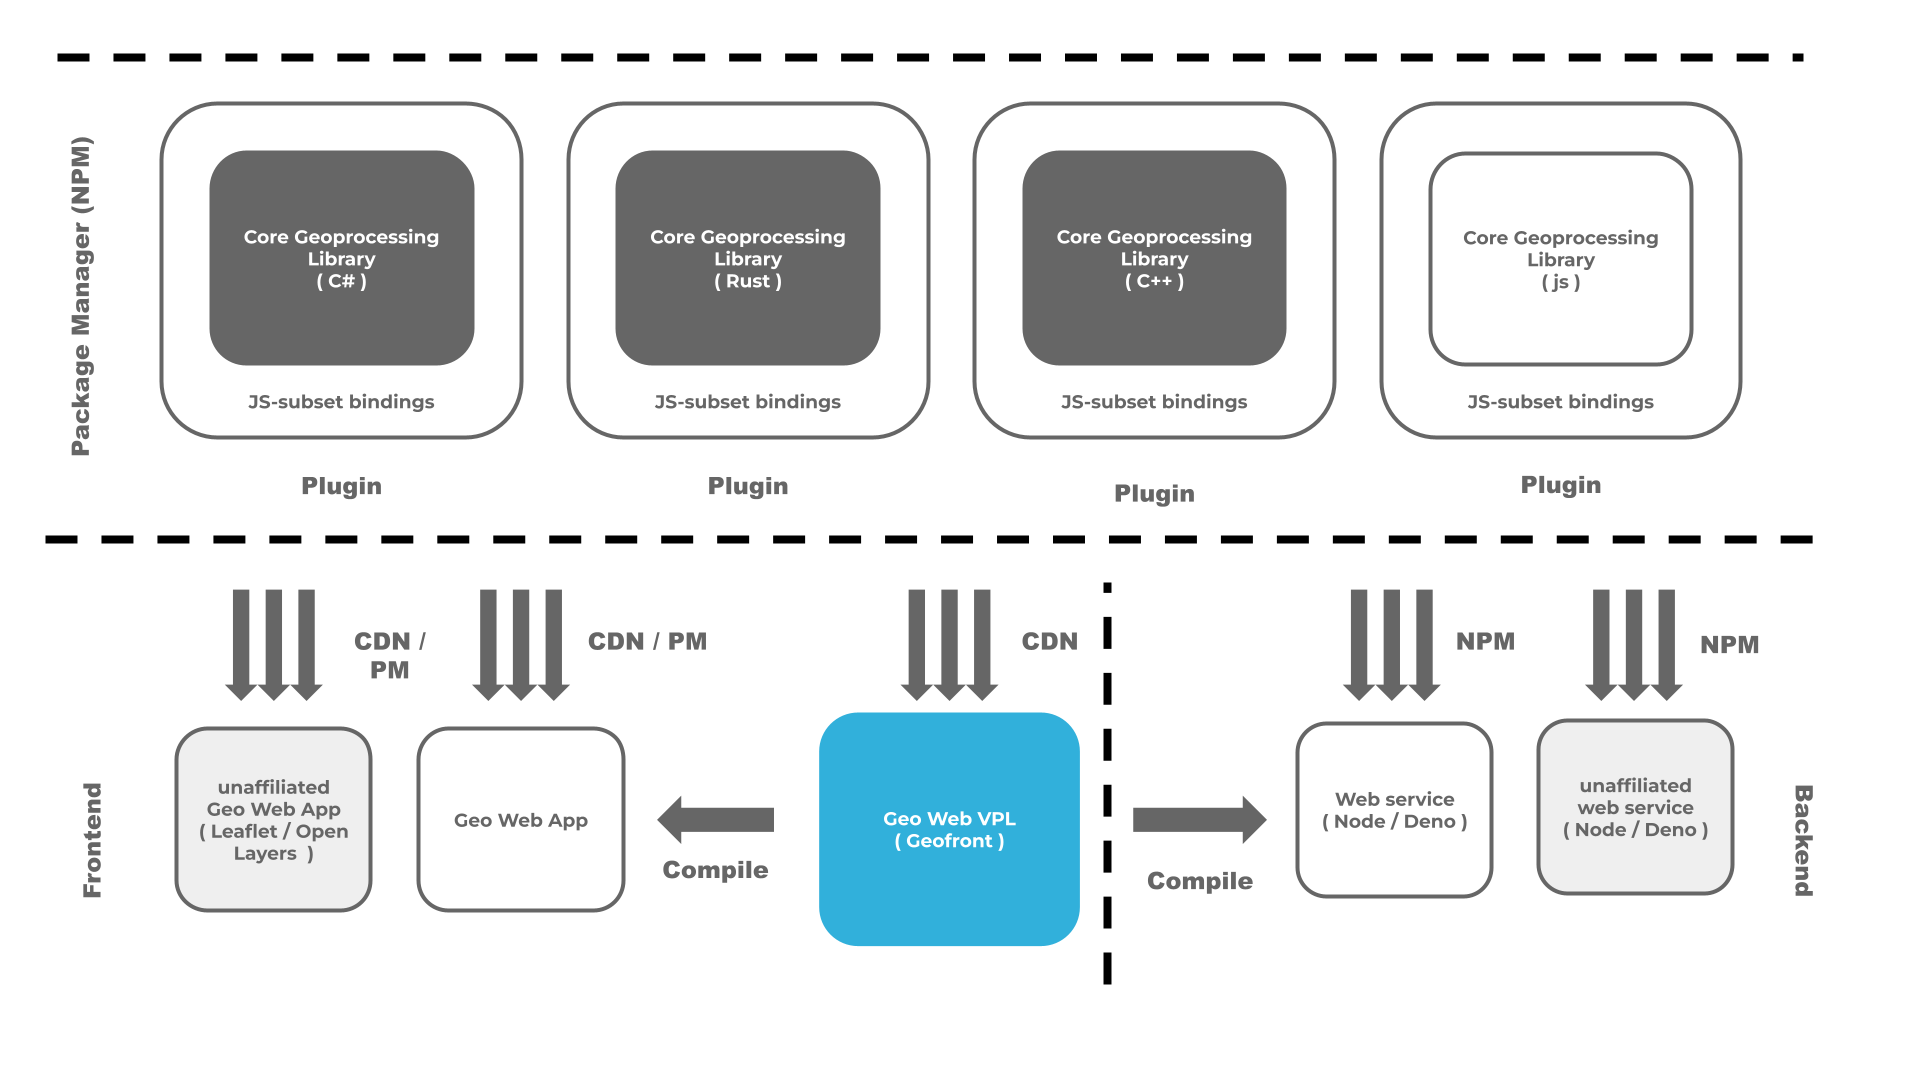
\includegraphics[width=\linewidth]{Model Proposal.png}
  \caption{Plugin Design}
  \label{fig:plugin-model}
\end{figure}

The components mentioned above fit together to propose the following workflow to use a native geo-library in a Web VPL: 
\begin{enumerate}
  \item Write or find a geocomputation library written in either C++ or Rust. 
  \item Create a second library, in which a subset of this 
     library is flagged and wrapped as 'functions usable on the web'.
  \subitem Optional: Include metadata to add additional functionality to the library
  \item Compile this library with a compatible compiler.
  \item Publish the results of these compilers to a \ac{CDN}. 
  
  \item Within the VPL: Reference the CDN address to the plugin loader. 
  \item The plugin loader now loads and converts the exposed functions, and includes them in the list of VPL components, ready to be used in the VPL. 
\end{enumerate}
What follows is an elaboration on the side of the plugin model, and on the side of the plugin loader.

\subsection{Plugin Model}

The plugin model serves three purposes:

\subsubsection{Compilation}

One, it needs to form a bridge between the language in which the geocomputation library is written, and javascript. 
In other words, the requirements of the WebAssembly compiler compatible with the language in question must be adhered to. 
Both the C++ and Rust compilers require functions to be flagged explicitly for compilation. 
Additionally, for a library to be compilable, all dependent libraries must also be able to compile to wasm.
For C++, the Emscripten compiler can be used to compile to WebAssembly \citep*{emscripten_organization_emscripten_2022}. 
A minimum example of what a 'emscripten-ready-library' looks like can be seen in \reffig{fig:minimum-cpp-wasm}.

For Rust, the 'wasm-pack' and 'wasm-bindgen' toolkits enable \ac{wasm} compilation \citep{contributors_wasm-bindgen_2022,contributors_wasm-pack_2022}.
A minimum example of what this looks like can be seen in \reffig{fig:minimum-rust-wasm}.
These toolkits do not require incremental compilation steps.
What is needed, however, is to make sure all dependencies do not use incompatible features, like os file system access. 
Fortunately, most Rust libraries are written with 'no-std' use-cases in mind, and contain flags to easily exclude these features. 

\begin{figure}
  \centering
  \graphicspath{ {../../assets/images/misc/} }
  
\includegraphics[width=\linewidth]{placeholder.png}
  \caption{TODO:  C++: Minimum WebAssembly example}
  \label{fig:minimum-cpp-wasm}
\end{figure}

\begin{figure}
  \centering
  \graphicspath{ {../../assets/images/misc/} }
  
\includegraphics[width=\linewidth]{placeholder.png}
  \caption{TODO: Rust: Minimum WebAssembly example}
  \label{fig:minimum-rust-wasm}
\end{figure}

\begin{figure}
  \centering
  \graphicspath{ {../../assets/images/misc/} }
  
\includegraphics[width=\linewidth]{placeholder.png}
  \caption{TODO: Rust: Exclude std features}
  \label{fig:minimum-rust-wasm-no-std}
\end{figure}

\subsubsection{Wrapping}

Two, it needs to bridge the gap between the dataflow-VPL and regular software library on a functional level. 
This comes down to wrapping the functionality of the geocomputation library as pure functions. 
This often leads to making copies of inputs / outputs, or grouping a series of steps to make an imperative interface functional (See \reffig{fig:oop-considered-harmful})

\begin{figure}
  \centering
  \graphicspath{ {../../assets/images/6/3/} }
  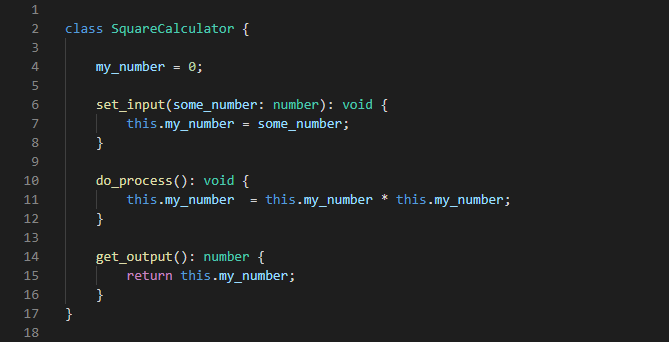
\includegraphics[width=\linewidth]{ugly-oop.png}
  \caption[]{This typescript is written in a non-functional manner, troubling its conversion to the functional model used by a dataflow VPL}
  \label{fig:oop-considered-harmful}
\end{figure}

\subsubsection{Flagging}

And Three, it need to communicate the content of the plugin to the VPL. 
We distinguish between \emph{required} data, and \emph{optional data}.
The central idea for this aspect is to generate this information automatically from the wasm binary and related files.
Only when that is impossible, should the information be manually hardcoded within the plugin.

The following information is \emph{required} for the VPL to load a geocomputation library, and convert it into visual components:

\begin{enumerate}[-]
  \item A list of all functions present in the library, uniquely named.
  \item A list of all custom types (structs / classes) present in the library, also uniquely named.
  \item Per function:  
  \subitem A list of all input parameters, name and type.
  \subitem An output type.
\end{enumerate}

The following information is \emph{optional}, but it would improve the functionality and usability of the library:
\begin{enumerate}[-]
  \item Per function:
  \subitem A custom, human-readable name.
  \subitem A description to explain usage.

  \item Per type:
  \subitem A custom, human-readable name.
  \subitem A description to explain usage.
  \subitem Functions for serializing and deserializing this type (binary, json)  
  \subitem Functions for rendering this type in 2D or 3D.
  \subitem A 'constructor' and 'deconstructor', to convert this type from and to basic types present within the VPL.  
\end{enumerate}

% \begin{figure}
%   \centering
%   \graphicspath{ {../../assets/diagrams/} }
%   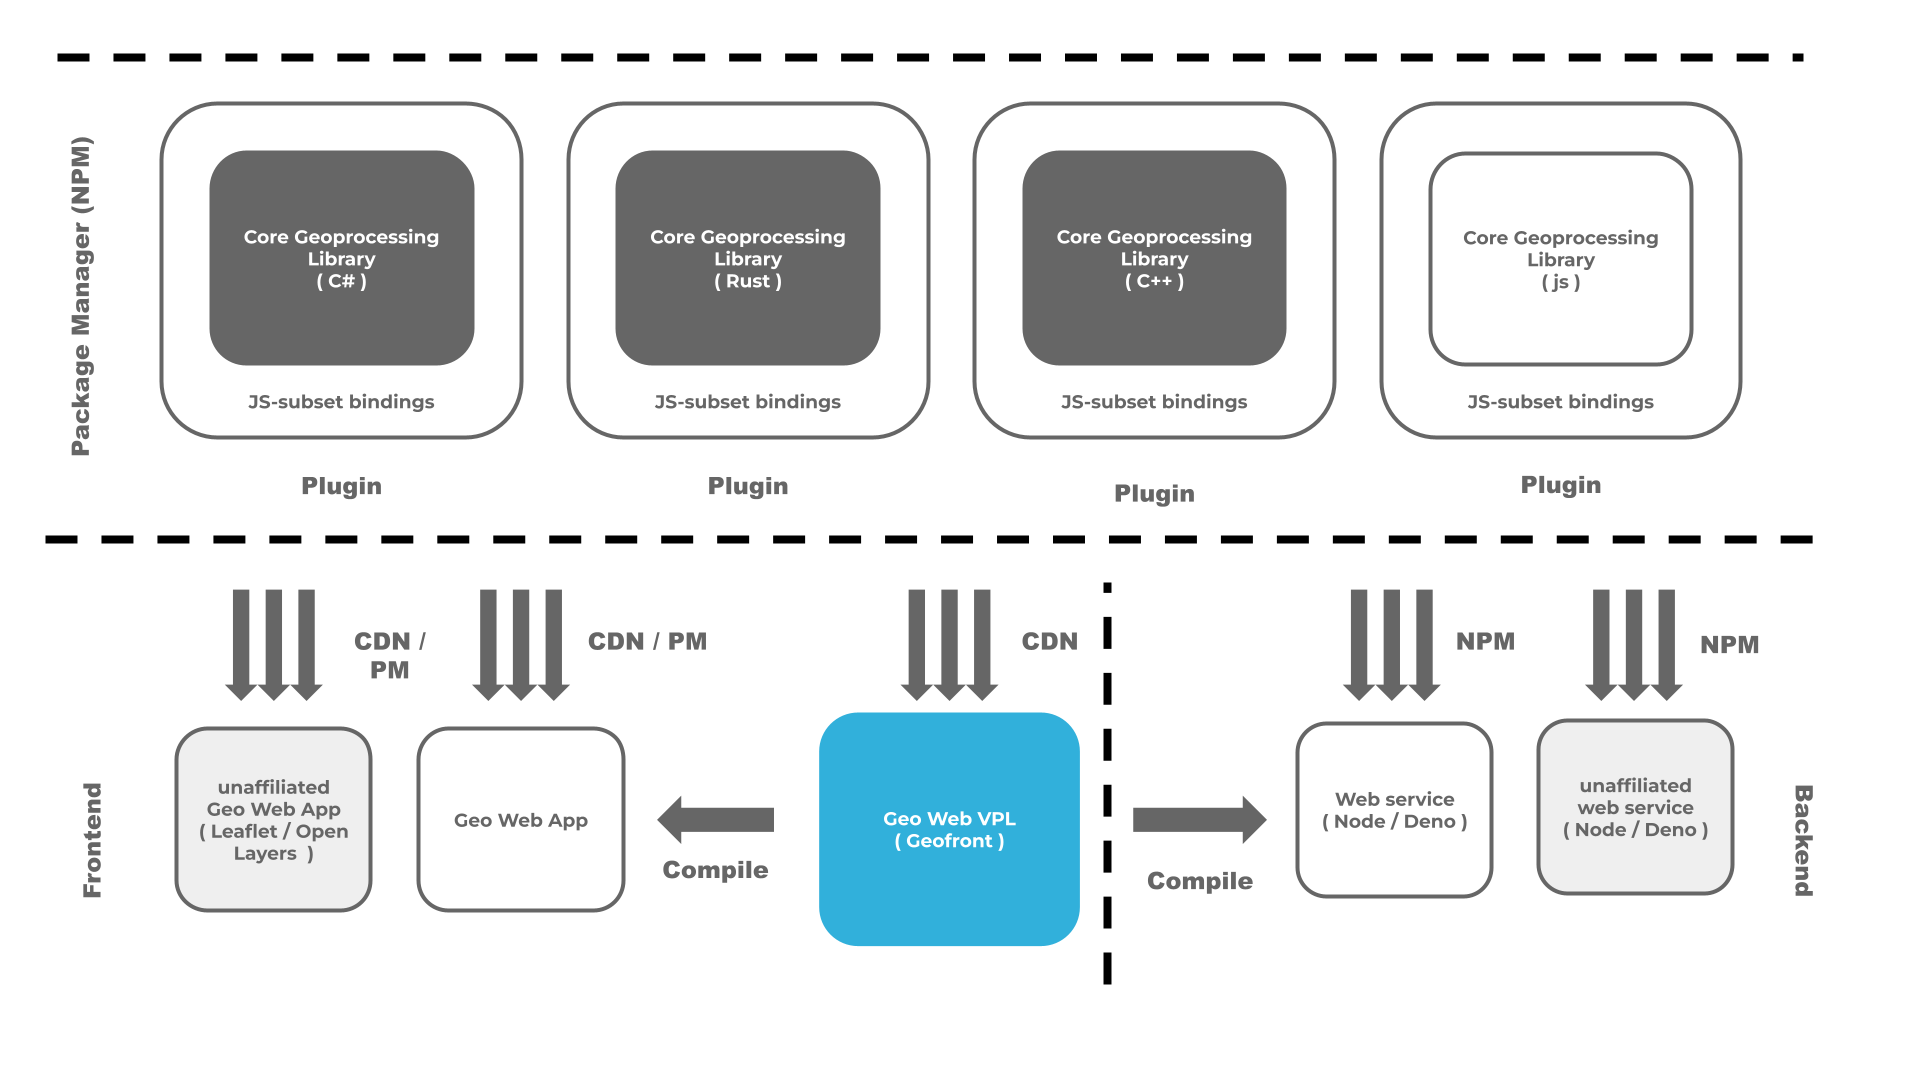
\includegraphics[width=\linewidth]{Model Proposal.png}
%   \caption{TODO: Proposed Plugin model with flagged functions}
%   \label{fig:plugin-model}
% \end{figure}

% \subsection{Plugin Loader}

% \begin{figure}
%   \centering
%   \graphicspath{ {../../assets/diagrams/} }
%   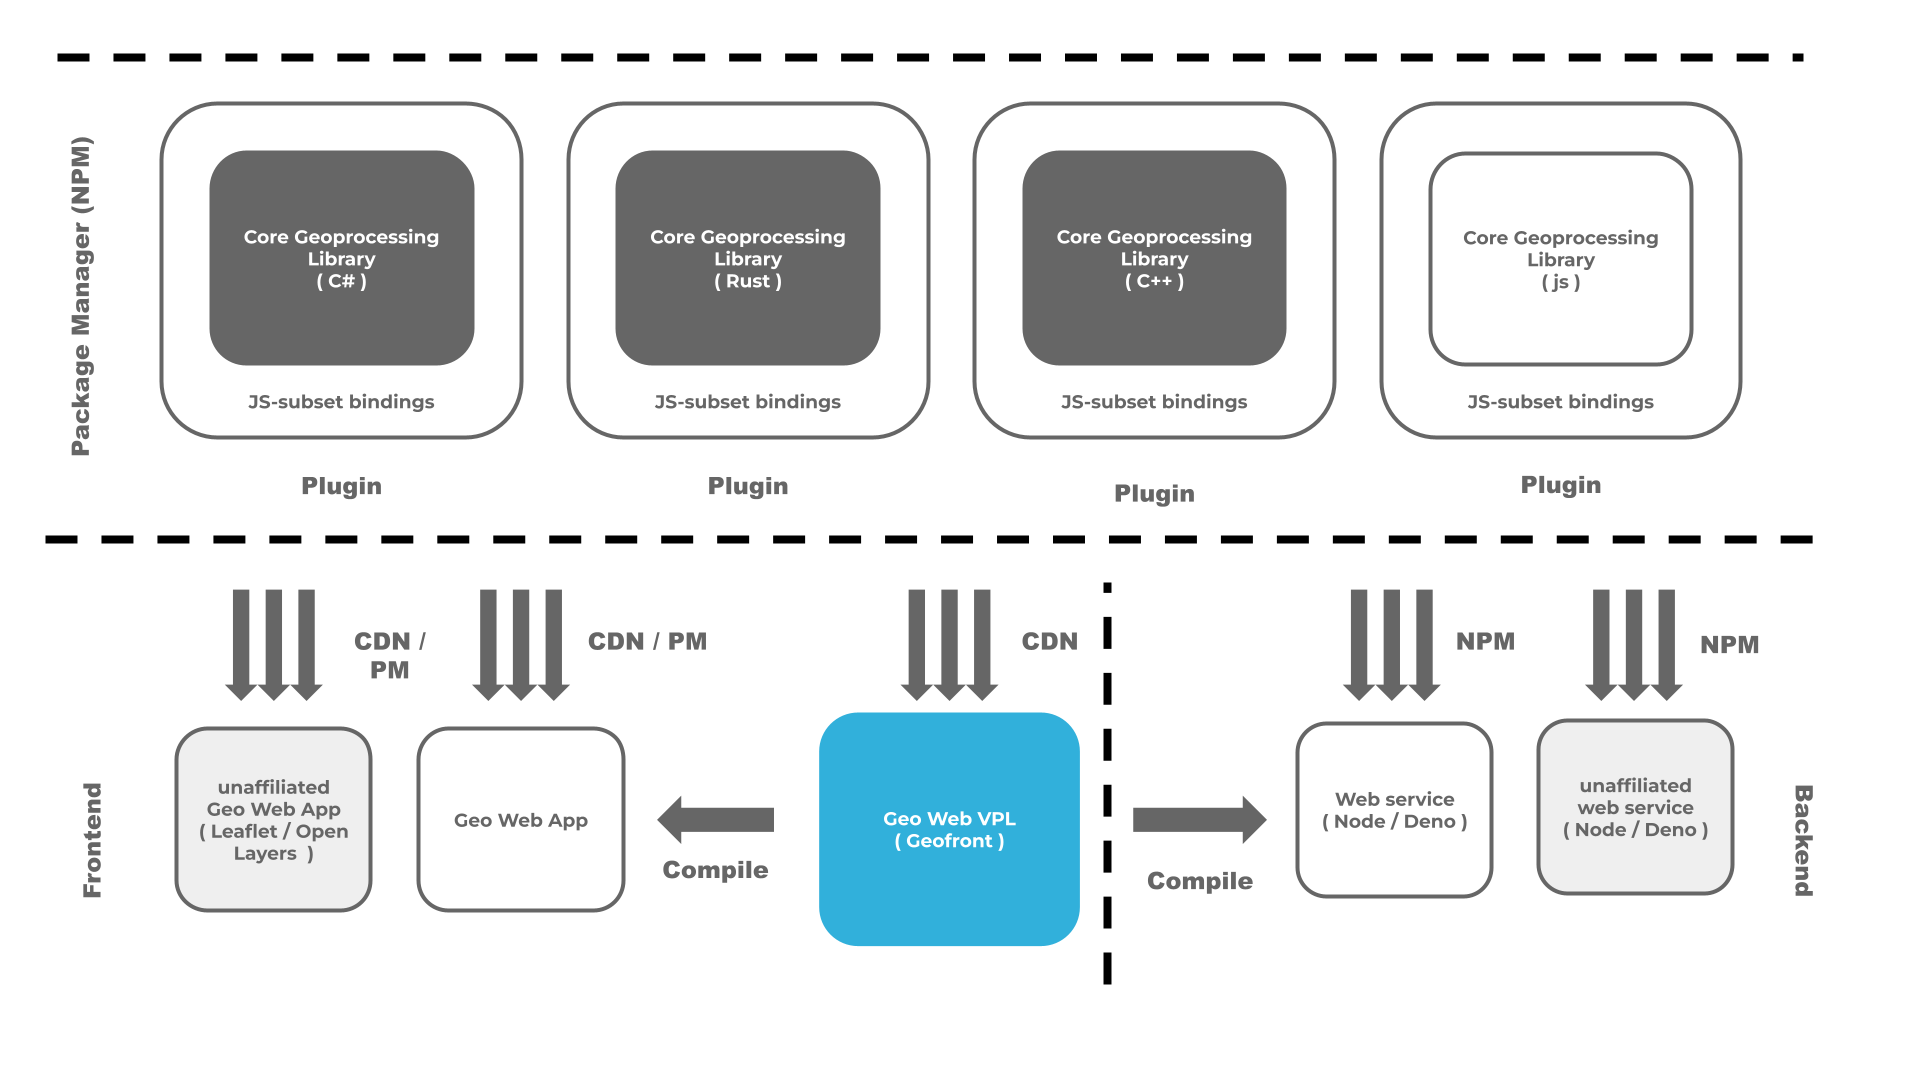
\includegraphics[width=\linewidth]{Model Proposal.png}
%   \caption{TODO: javascript \& d.ts headers}
%   \label{fig:plugin-model}
% \end{figure}

On the side of the plugin loader within the VPL, all the compiled, wrapped and flagged information within the plugin needs to be extracted. 
The automated extraction of all \textbf{required} information can be done by utilizing TypeScript Declaration 'd.ts' files. 
A 'd.ts' file can be understood as a 'header' file generated by the TypeScript compiler, exposing the types required by all functions found in a corresponding javascript file.
By using the typescript compiler in the VPL, this header file could be loaded and interpreted to find all basic information, including the names, the namespace where to find a functions, and all input and output types.
This extraction of types was required, since these are not present in javascript source code, and types are needed in explaining to the end-user how to use a function, and in making the VPL typesafe.

With the extracted information from the "d.ts" file, a corresponding Javascript file can be traversed and loaded as a VPL plugin. 
javascript's nature as a scripting language can be utilized for this:
Firstly, its dynamic nature allowed a library to be loaded and incorporated at runtime without any special alterations. 
Hot-loading libraries in C++ for example, can't usually be done without significantly altering the way a program runs. 
Secondly, javascript's prototype-based classes and its support for reflection allows a plugin loader to localize and collect all functions within a library.
And lastly, the "first-class function support" allowed these functions to be referenced and called by the Nodes of the VPL Graph. 

Because the VPL will be implemented as a Dataflow-VPL, the loader seeks to extract only (pure) functions. 
However, many libraries also include classes, as these can make an API more clear to use using regular languages. 
The plugin loader will need to support classes by converting them to a series of normal functions. 
Static methods and constructors can be converted directly, and methods are converted into functions with the object as the first argument.

The \textbf{optional} data can be exposed by flagging functions with a standard prefix.
These functions are then loaded by the vpl, but will not be converted into visual components. 
Instead, these functions are programmatically called when the VPL engine or the user requires this optional aspect. 

%%%%%%%%%%%%%%%%%%%%%%%%%%%%%%%%%%%%%%%%%%%%%%%%%%%%%%%%%%%%%%%%%%%%%%%%%%%%%%%
%%%%%%%%%%%%%%%%%%%%%%%%%%%%%%%%%%%%%%%%%%%%%%%%%%%%%%%%%%%%%%%%%%%%%%%%%%%%%%%
%%%%%%%%%%%%%%%%%%%%%%%%%%%%%%%%%%%%%%%%%%%%%%%%%%%%%%%%%%%%%%%%%%%%%%%%%%%%%%%
%%%%%%%%%%%%%%%%%%%%%%%%%%%%%%%%%%%%%%%%%%%%%%%%%%%%%%%%%%%%%%%%%%%%%%%%%%%%%%%
%%%%%%%%%%%%%%%%%%%%%%%%%%%%%%%%%%%%%%%%%%%%%%%%%%%%%%%%%%%%%%%%%%%%%%%%%%%%%%%

\newpage
\section{Tests}
\label{sec:method:tests}
% The purpose of this final step of the methodology
With both the VPL and the plugin system in place, the final step of the methodology is introduced to gather the results and data needed for properly answering the second, third fourth sub-research questions.

% \begin{note}
%   - see how well the plugin system is able to handle C++ and Rust native libraries. 
%   - see how usable the resulting applications created within the VPL are.     
% \end{note}

\subsection{Compilation Tests}
To test the ability of the VPl and the plugin system to host different libraries and different languages, four demo plugins are compiled and loaded within the VPL.  
The Rust language and C++ are tested. 
Per test, the workflow layed out in \refsec{sec:method:plugin-system} is followed. 
Per language, a minimum plugin is first created, assessing if and how well a simple function, method, and class can be exposed to the VPL.
After this demo, a more sizable, existing geocomputation library is compiled.

These tests are meant as a qualitative comparison between compiling a full-scale library written in Rust, to a full library written in C++. 
This way, the tooling and workflow can be compared for a realistic use-case. 
The study is conducted by compiling both libraries using their respective \ac{wasm} toolsets, and noting the differences in workflow, supported features, and the resulting plugins. 

The libraries must be compiled without 'disruption': They must be kept the exact same for normal, native usage. 

\begin{note}
  HUGO: GDAL-JS ???
    L takes some time to convert it to a functional model
    L cannot be used by the plugin system directly, but can be used as a dependency in geofront itself.
  STARTIN: small s

\end{note}

\subsubsection{C++ Library: CGAL} 
The library tested for C++ is CGAL, compiled using \m{emscriptem}. 
For one, this library is well established and very relevant to geoprocessing as a whole. 
Many other C++ geo-libraries depend on it.
Moreover, it is a sizable and complex project, making it highly likely the problems described by \refsec{sec:background-wasm} are encountered. 
We could choose more simple libraries, but this is not representative of most C++ geoprocessing libraries. 

\subsubsection{Rust Library: Startin}
The second library tested is the Startin library, written in Rust, compiled using \m{wasm-bindgen}.  
This library is smaller in scope than CGAL. 
Ideally, a library with a size comparable to CGAL should have been chosen, to make for a balanced comparison. 
However, Rust is still a relatively unknown language in the field of GIS, making libraries like these difficult to find. 
Startin was chosen, for the triangulation functionalities it provides makes for a good comparison against CGALs Triangulator. 
It also, just like CGAL, makes use of a high precision kernel, and offers geometric robustness. 


% This will be done by using the VPL and plugin loader to create an application. 
% This application, and the process to create it, will then be assessed.

% \subsubsection{Application}

% \begin{note}
% TODO: make a point cloud -> dtm obj tool / isocurves svg / tool
% \end{note}

% \subsubsection{First Experiment}
% The first experiment compares three different methods of bringing the same geocomputation procedure to the web. 
% This way, quantitative, measurable aspects of these methods can be compared. 
% The following three methods are tested:
% \begin{enumerate}[-]
%   \item Write the procedure in normal javascript
%   \item Write the procedure in C++, compile to wasm using the \m{emscriptem} toolkit (Source)
%   \item Write the procedure in Rust, compile to wasm using the \m{wasm-bindgen} toolkit (Source)
% \end{enumerate}
% These procedures are all tested within the same web application, using the same data. 
% By taking two different languages, we can distinguish between shortcomings of \ac{wasm} itself, and the \ac{wasm} support of a language.  

% The procedure chosen is a 2D convex hull calculation of a set of sample points. 
% The chosen procedure must be small enough to clearly reason about performance differences, and yet large enough to pose a substantial computational challenge, validating the usage of \ac{wasm}.

% \begin{note}
%   Expand upon the procedure
% \end{note}

% The three methods will be compared in terms of:
% \begin{enumerate}[-]
%   \item performance
%   \item load times
%   \item memory usage
% \end{enumerate}

% \begin{note}
%   - todo: turn features around into assessment criteria
%   - performance: load times, run times
%   - current state of webassembly & js. how much faster is it? is it even faster? 
%      - data translation steps, do they mitigate performance gains? 
%      - also given the fact that we are doing 'functions on sets'/ declarative instead of imperative styles, forced by the format of dataflow programming. 
% \end{note}

% The studies on browser-based geocomputation (\refsec{sec:related-geoweb}) appear to have conducted a similar experiment, by comparing the same procedure written in C++ and javascript. 
% However, these studies compared javascript against a native, non-web compilation of C++. 
% This experiment also differs in distinguishing between \ac{wasm} itself, and a language's \ac{wasm} support.

% %%%%%%%%%%%%%%%%%%%%%%%%%%%%%%%%%%%%%%%%%%%%%%%%%%%%%%%%%%%%%%%%%%%%%%%%%%%%%%%

% \subsubsection{Second Experiment

\subsection{Usage tests}

% The second set of tests seek the data needed to answer the question of \mySubRQFourTitle: \mySubRQFour.
To acquire this data, an application will be created using the VPL, which will be subjected to a qualitative assessment. 

\subsubsection{Feature Assessment}

\emph{Per requirement, to what extent is it successfully implemented by this dataflow-VPL?}.
\emph{Per requirement, which role did the core browser features play in supporting or hindering it?}.

\subsubsection{Assessment Framework}
For the assessment criteria, the cognitive dimensions framework of \cite[]{green_usability_1996} will be used. 
The framework is useful for its focus on language features. 
This allows the assessment to be made within the scope of this study, and without performing user-testing.
Also, as commented on in \refsec{sec:background-vpl}, the study has acquired a canonical nature among many VPL researchers for its elaborate examination of the "Psychology of Programming".
The age of the study indicates that the principles have stood the test of time. 

The framework presents the following 13 dimensions and accompanying descriptions \cite[]{green_usability_1996}:
\begin{enumerate}
  \item Abstraction gradient: What are the minimum and maximum levels of abstraction? Can fragments be encapsulated? 

  \item Closeness of mapping: What 'programming games' need to be learned? 
  
  \item Consistency: When some of the language has been learnt, how much of the rest can be inferred? 
  
  \item Diffuseness: How many symbols or graphic entities are required to express a meaning? 
  
  \item Error- proneness: Does the design of the notation induce 'careless mistakes'? 
  
  \item Hard mental operations: Are there places where the user needs to resort to fingers or pencilled annotation to keep track of what's happening? 
  
  \item Hidden dependencies: Is every dependency overtly indicated in both directions? Is the indication perceptual or only symbolic? 
  
  \item Premature commitment: Do programmers have to make decisions before they have the information they need? 
  
  \item Progressive evaluation: Can a partially-complete program be executed to obtain feedback on 'How am I doing'? 
  
  \item Role- expressiveness: Can the reader see how each component of a program relates to the whole? 
  
  \item Secondary notation: Can programmers use layout, colour, other cues to convey extra meaning, above and beyond the 'official' semantics of the language? 
  
  \item Viscosity: How much effort is required to perform a single change? 
  
  \item Visibility: Is every part of the code simultaneously visible (assuming a large enough display), or it it at least possible to juxtapose any two parts side-by-side at will? If the code is dispersed, is it at least possible to know in what order to read it?
\end{enumerate}

As stated by the authors; the purpose of this framework is to make the trade-offs chosen by a language's designer explicit. It is not meant as a 'scoring' system.


%%%%%%%%%%%%%%%%%%%%%%%%%%%%%%%%%%%%%%%%%%%%%%%%%%%%%%%%%%%%%%%%%%%%%%%%%%%%%%%
%%%%%%%%%%%%%%%%%%%%%%%%%%%%%%%%%%%%%%%%%%%%%%%%%%%%%%%%%%%%%%%%%%%%%%%%%%%%%%%
%%%%%%%%%%%%%%%%%%%%%%%%%%%%%%%%%%%%%%%%%%%%%%%%%%%%%%%%%%%%%%%%%%%%%%%%%%%%%%%
%%%%%%%%%%%%%%%%%%%%%%%%%%%%%%%%%%%%%%%%%%%%%%%%%%%%%%%%%%%%%%%%%%%%%%%%%%%%%%%
%%%%%%%%%%%%%%%%%%%%%%%%%%%%%%%%%%%%%%%%%%%%%%%%%%%%%%%%%%%%%%%%%%%%%%%%%%%%%%%

%%%%%%%%%%%%%%%%%%%%%%%%%%%%%%%%%%%%%%%%%%%%%%%%%%%%%%%%%%%%%%%%%%%%%%%%%%%%%%%
%%%%%%%%%%%%%%%%%%%%%%%%%%%%%%%%%%%%%%%%%%%%%%%%%%%%%%%%%%%%%%%%%%%%%%%%%%%%%%%
%%%%%%%%%%%%%%%%%%%%%%%%%%%%%%%%%%%%%%%%%%%%%%%%%%%%%%%%%%%%%%%%%%%%%%%%%%%%%%%
%%%%%%%%%%%%%%%%%%%%%%%%%%%%%%%%%%%%%%%%%%%%%%%%%%%%%%%%%%%%%%%%%%%%%%%%%%%%%%%
%%%%%%%%%%%%%%%%%%%%%%%%%%%%%%%%%%%%%%%%%%%%%%%%%%%%%%%%%%%%%%%%%%%%%%%%%%%%%%%


%% OLD STUFF



%%%%%%%%%%%%%%%%%%%%%%%%%%%%%%%%%%%%%%%%%%%%%%%%%%%%%%%%%%%%%%%%%%%%%%%%%%%%%%%

%%%%%%%%%%%%%%%%%%%%%%%%%%%%%%%%%%%%%%%%%%%%%%%%%%%%%%%%%%%%%%%%%%%%%%%%%%%%%%%






% \begin{enumerate}[-]
%   \item Develop a representative use-case application within the prototype \ac{geo-web-vpl}.
%   \item Develop a command line application capable of the very same process.
%   \item Assess both applications according to a series of assessment questions.
% \end{enumerate}

% The execution of this component of the methodology is found in \refsec{sec:analyses:utilization}.

% \subsection{use-case application}
% The application used in both test cases is an "isocurves from DTM" process. 
% But also: we want the iso-curves of a specific location. How to get this data is part of the exercise

% \begin{note}
% [This is subject to change, according to how much I can accomplish ]

% - find the required height data as WFS / WMS
% - determine a boundary
% - load a dtm as a regular png / tiff image
% - specify the parameters, like height delta, smoothness.
% - marching squares
% - post-process curves
% - save as wkt, geojson, or some other well-known vector format

% \end{note}

% Nielsen and Molichs 10 User Interface Design Guidelines
% https://theomandel.com/resources/golden-rules-of-user-interface-design/
% https://www.interaction-design.org/literature/article/user-interface-design-guidelines-10-rules-of-thumb
% (old rules, but still relevant)_
